\documentclass[tikz,border=0pt]{standalone}
\usepackage{xcolor}
\usetikzlibrary{calc}
% Palette: Sam_Comm_final.png by eye, and the drones and raiders.
\definecolor{ink}{HTML}{3B2340}
\definecolor{sky}{HTML}{EFC46A}
\definecolor{skyhi}{HTML}{F5DA92}
\definecolor{skylow}{HTML}{E9B060}
\definecolor{cloud}{HTML}{F2D58A}
\definecolor{paper}{HTML}{FBEFD0}
\definecolor{cream}{HTML}{FFF6E0}
\definecolor{white}{HTML}{FFFFFF}
\definecolor{wallA}{HTML}{E88A73}
\definecolor{wallB}{HTML}{EE9F7E}
\definecolor{wallC}{HTML}{E47A7E}
\definecolor{wallD}{HTML}{F0B07E}
\definecolor{wallE}{HTML}{D9765F}
\definecolor{wallF}{HTML}{E99A8A}
\definecolor{greenA}{HTML}{8DBB7E}
\definecolor{greenB}{HTML}{6FA77A}
\definecolor{greenC}{HTML}{A9C97F}
\definecolor{greenD}{HTML}{5E9C6A}
\definecolor{greenE}{HTML}{4A8060}
\definecolor{sage}{HTML}{9DB98A}
\definecolor{sagedark}{HTML}{6F8F66}
\definecolor{sagelight}{HTML}{C2D6A6}
\definecolor{window}{HTML}{F6E7A0}
\definecolor{windark}{HTML}{8C5A64}
\definecolor{metal}{HTML}{8D9A93}
\definecolor{metaldark}{HTML}{5E6B66}
\definecolor{metallight}{HTML}{B9C4BC}
\definecolor{wood}{HTML}{B9835A}
\definecolor{wooddark}{HTML}{8C5A3C}
\definecolor{woodlight}{HTML}{D9A66F}
\definecolor{stone}{HTML}{E7C9A0}
\definecolor{stonedark}{HTML}{C9A47E}
\definecolor{concrete}{HTML}{D8C3A4}
\definecolor{concretedark}{HTML}{B8A084}
\definecolor{asphalt}{HTML}{8E7A86}
\definecolor{asphaltdark}{HTML}{6E5C68}
\definecolor{roadline}{HTML}{F6E7A0}
\definecolor{kerb}{HTML}{D8B48C}
\definecolor{red}{HTML}{E0483E}
\definecolor{redlight}{HTML}{F27A6A}
\definecolor{gold}{HTML}{FFB000}
\definecolor{goldlight}{HTML}{FFD54F}
\definecolor{teal}{HTML}{4FA3A0}
\definecolor{tealdark}{HTML}{3C8582}
\definecolor{magenta}{HTML}{FF2E88}
\definecolor{cyan}{HTML}{13CFE3}
\definecolor{violet}{HTML}{8A5BD6}
\definecolor{orange}{HTML}{F2803A}
\definecolor{pink}{HTML}{F48FB1}
\definecolor{glow}{HTML}{4FE6E0}
\definecolor{glowhi}{HTML}{C8FFF9}
\definecolor{hot}{HTML}{FF6A1A}
\definecolor{hothi}{HTML}{FFD07A}
\definecolor{armour}{HTML}{7E7A86}
\definecolor{armourdark}{HTML}{5A5466}
\definecolor{armourlight}{HTML}{A8A2B0}
\definecolor{wasp}{HTML}{E0A82E}
\definecolor{waspdark}{HTML}{B07E1A}
\definecolor{moth}{HTML}{F2E6C8}
\definecolor{mothdark}{HTML}{D2C09A}
\definecolor{hornet}{HTML}{3C8582}
\definecolor{hornetdark}{HTML}{2C6260}
\definecolor{warden}{HTML}{E47A7E}
\definecolor{wardendark}{HTML}{B85A62}
\definecolor{tick}{HTML}{8DBB7E}
\definecolor{tickdark}{HTML}{5E8A5A}
\definecolor{strider}{HTML}{D9765F}
\definecolor{striderdark}{HTML}{A8543F}
\definecolor{jacket}{HTML}{6FA77A}
\definecolor{jacketb}{HTML}{4FA3A0}
\definecolor{jacketc}{HTML}{E88A73}
\definecolor{jacketd}{HTML}{F0B07E}
\definecolor{skin}{HTML}{F2C49A}
\definecolor{skinb}{HTML}{C98C6A}
\definecolor{skinc}{HTML}{8C5A3C}
\definecolor{hair}{HTML}{3B2340}
\definecolor{goo}{HTML}{B6E35A}
\definecolor{goodark}{HTML}{7FB23A}
\newcommand{\Ink}{1.15pt}
\tikzset{inked/.style={draw=ink, line width=\Ink, line join=round, line cap=round}}
\begin{document}
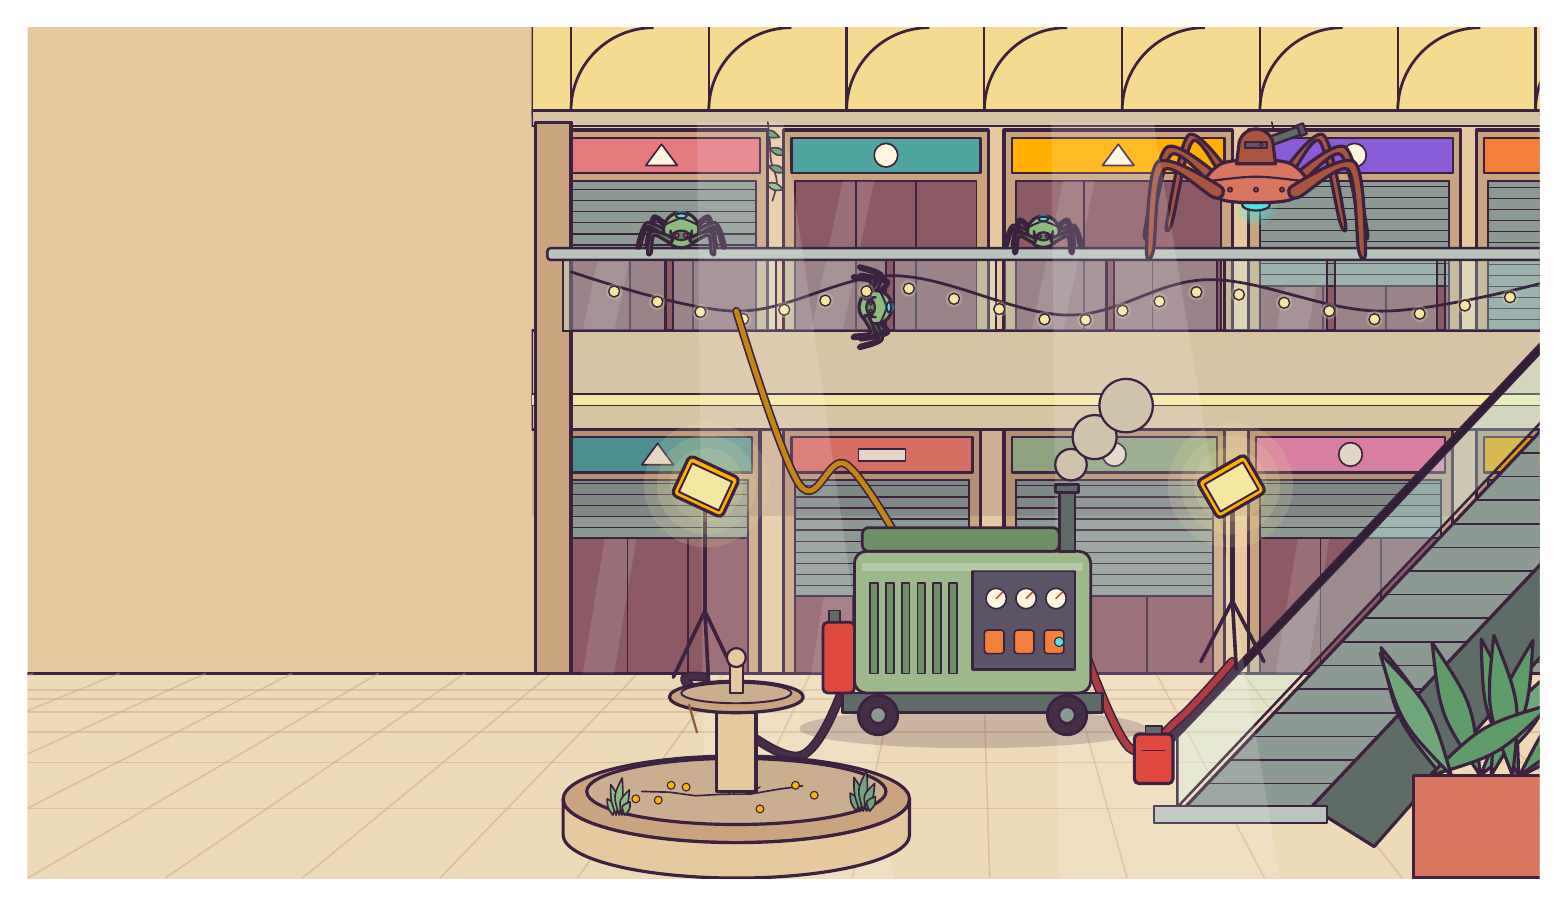
\begin{tikzpicture}
\clip (0,0) rectangle (19.2,10.8);
\filldraw[inked,fill=stone] (-0.5,-0.5) rectangle (19.7,11.3);
\filldraw[inked,fill=paper!65!kerb] (-0.5,-0.5) rectangle (19.7,2.6);
\draw[ink, line width=1.1pt, line cap=round] (-0.5,2.6) -- (19.7,2.6);
\draw[stonedark, opacity=0.45, line width=0.6pt] (-19.2,0) -- (-7.611,2.6);
\draw[stonedark, opacity=0.45, line width=0.6pt] (-17.455,0) -- (-6.514,2.6);
\draw[stonedark, opacity=0.45, line width=0.6pt] (-15.709,0) -- (-5.417,2.6);
\draw[stonedark, opacity=0.45, line width=0.6pt] (-13.964,0) -- (-4.32,2.6);
\draw[stonedark, opacity=0.45, line width=0.6pt] (-12.218,0) -- (-3.223,2.6);
\draw[stonedark, opacity=0.45, line width=0.6pt] (-10.473,0) -- (-2.126,2.6);
\draw[stonedark, opacity=0.45, line width=0.6pt] (-8.727,0) -- (-1.029,2.6);
\draw[stonedark, opacity=0.45, line width=0.6pt] (-6.982,0) -- (0.069,2.6);
\draw[stonedark, opacity=0.45, line width=0.6pt] (-5.236,0) -- (1.166,2.6);
\draw[stonedark, opacity=0.45, line width=0.6pt] (-3.491,0) -- (2.263,2.6);
\draw[stonedark, opacity=0.45, line width=0.6pt] (-1.745,0) -- (3.36,2.6);
\draw[stonedark, opacity=0.45, line width=0.6pt] (0,0) -- (4.457,2.6);
\draw[stonedark, opacity=0.45, line width=0.6pt] (1.745,0) -- (5.554,2.6);
\draw[stonedark, opacity=0.45, line width=0.6pt] (3.491,0) -- (6.651,2.6);
\draw[stonedark, opacity=0.45, line width=0.6pt] (5.236,0) -- (7.749,2.6);
\draw[stonedark, opacity=0.45, line width=0.6pt] (6.982,0) -- (8.846,2.6);
\draw[stonedark, opacity=0.45, line width=0.6pt] (8.727,0) -- (9.943,2.6);
\draw[stonedark, opacity=0.45, line width=0.6pt] (10.473,0) -- (11.04,2.6);
\draw[stonedark, opacity=0.45, line width=0.6pt] (12.218,0) -- (12.137,2.6);
\draw[stonedark, opacity=0.45, line width=0.6pt] (13.964,0) -- (13.234,2.6);
\draw[stonedark, opacity=0.45, line width=0.6pt] (15.709,0) -- (14.331,2.6);
\draw[stonedark, opacity=0.45, line width=0.6pt] (17.455,0) -- (15.429,2.6);
\draw[stonedark, opacity=0.45, line width=0.6pt] (19.2,0) -- (16.526,2.6);
\draw[stonedark, opacity=0.45, line width=0.6pt] (20.945,0) -- (17.623,2.6);
\draw[stonedark, opacity=0.45, line width=0.6pt] (22.691,0) -- (18.72,2.6);
\draw[stonedark, opacity=0.45, line width=0.6pt] (24.436,0) -- (19.817,2.6);
\draw[stonedark, opacity=0.45, line width=0.6pt] (26.182,0) -- (20.914,2.6);
\draw[stonedark, opacity=0.45, line width=0.6pt] (27.927,0) -- (22.011,2.6);
\draw[stonedark, opacity=0.45, line width=0.6pt] (29.673,0) -- (23.109,2.6);
\draw[stonedark, opacity=0.45, line width=0.6pt] (31.418,0) -- (24.206,2.6);
\draw[stonedark, opacity=0.45, line width=0.6pt] (33.164,0) -- (25.303,2.6);
\draw[stonedark, opacity=0.45, line width=0.6pt] (34.909,0) -- (26.4,2.6);
\draw[stonedark, opacity=0.45, line width=0.6pt] (36.655,0) -- (27.497,2.6);
\draw[stonedark, opacity=0.45, line width=0.6pt] (38.4,0) -- (28.594,2.6);
\draw[stonedark, opacity=0.45, line width=0.6pt] (-1,0.884) -- (20.2,0.884);
\draw[stonedark, opacity=0.45, line width=0.6pt] (-1,1.467) -- (20.2,1.467);
\draw[stonedark, opacity=0.45, line width=0.6pt] (-1,1.853) -- (20.2,1.853);
\draw[stonedark, opacity=0.45, line width=0.6pt] (-1,2.107) -- (20.2,2.107);
\draw[stonedark, opacity=0.45, line width=0.6pt] (-1,2.274) -- (20.2,2.274);
\draw[stonedark, opacity=0.45, line width=0.6pt] (-1,2.385) -- (20.2,2.385);
\begin{scope}\clip (6.4,-1) rectangle (20.2,11.8);
\filldraw[inked,fill=skyhi] (6.4,9.7) rectangle (19.7,11.3);
\filldraw[inked,fill=concrete,line width=0.9pt] (6.4,9.55) rectangle (19.7,9.75);
\draw[ink, line width=1.0pt] (6.9,9.75) arc[start angle=180, end angle=90, radius=1.05];
\draw[ink, line width=0.8pt, line cap=round] (6.9,9.75) -- (6.9,10.9);
\draw[ink, line width=1.0pt] (8.65,9.75) arc[start angle=180, end angle=90, radius=1.05];
\draw[ink, line width=0.8pt, line cap=round] (8.65,9.75) -- (8.65,10.9);
\draw[ink, line width=1.0pt] (10.4,9.75) arc[start angle=180, end angle=90, radius=1.05];
\draw[ink, line width=0.8pt, line cap=round] (10.4,9.75) -- (10.4,10.9);
\draw[ink, line width=1.0pt] (12.15,9.75) arc[start angle=180, end angle=90, radius=1.05];
\draw[ink, line width=0.8pt, line cap=round] (12.15,9.75) -- (12.15,10.9);
\draw[ink, line width=1.0pt] (13.9,9.75) arc[start angle=180, end angle=90, radius=1.05];
\draw[ink, line width=0.8pt, line cap=round] (13.9,9.75) -- (13.9,10.9);
\draw[ink, line width=1.0pt] (15.65,9.75) arc[start angle=180, end angle=90, radius=1.05];
\draw[ink, line width=0.8pt, line cap=round] (15.65,9.75) -- (15.65,10.9);
\draw[ink, line width=1.0pt] (17.4,9.75) arc[start angle=180, end angle=90, radius=1.05];
\draw[ink, line width=0.8pt, line cap=round] (17.4,9.75) -- (17.4,10.9);
\draw[ink, line width=1.0pt] (19.15,9.75) arc[start angle=180, end angle=90, radius=1.05];
\draw[ink, line width=0.8pt, line cap=round] (19.15,9.75) -- (19.15,10.9);
\draw[ink, line width=0.6pt, line cap=round, line join=round] plot[smooth, tension=0.6] coordinates {(9.4,9.6) (9.426,9.35) (9.442,9.1) (9.514,8.85) (9.457,8.6)};
\filldraw[inked,fill=greenD,line width=0.6pt] (9.329,9.489) .. controls (9.46,9.505) .. (9.549,9.409) .. controls (9.419,9.393) .. (9.329,9.489) -- cycle;
\filldraw[inked,fill=greenB,line width=0.6pt] (9.36,9.378) .. controls (9.271,9.281) .. (9.14,9.298) .. controls (9.23,9.394) .. (9.36,9.378) -- cycle;
\filldraw[inked,fill=greenD,line width=0.6pt] (9.419,9.267) .. controls (9.549,9.283) .. (9.639,9.187) .. controls (9.508,9.17) .. (9.419,9.267) -- cycle;
\filldraw[inked,fill=greenA,line width=0.6pt] (9.325,9.156) .. controls (9.236,9.059) .. (9.105,9.076) .. controls (9.195,9.172) .. (9.325,9.156) -- cycle;
\filldraw[inked,fill=greenD,line width=0.6pt] (9.407,9.044) .. controls (9.538,9.061) .. (9.627,8.964) .. controls (9.497,8.948) .. (9.407,9.044) -- cycle;
\filldraw[inked,fill=greenB,line width=0.6pt] (9.363,8.933) .. controls (9.273,8.837) .. (9.143,8.853) .. controls (9.232,8.95) .. (9.363,8.933) -- cycle;
\filldraw[inked,fill=greenA,line width=0.6pt] (9.376,8.822) .. controls (9.507,8.839) .. (9.596,8.742) .. controls (9.466,8.726) .. (9.376,8.822) -- cycle;
\filldraw[inked,fill=greenD,line width=0.6pt] (9.4,8.711) .. controls (9.31,8.615) .. (9.18,8.631) .. controls (9.269,8.727) .. (9.4,8.711) -- cycle;
\draw[ink, line width=0.6pt, line cap=round, line join=round] plot[smooth, tension=0.6] coordinates {(15.8,9.6) (15.853,9.25) (15.75,8.9) (15.785,8.55) (15.708,8.2)};
\filldraw[inked,fill=greenD,line width=0.6pt] (15.847,9.444) .. controls (15.977,9.461) .. (16.067,9.364) .. controls (15.936,9.348) .. (15.847,9.444) -- cycle;
\filldraw[inked,fill=greenD,line width=0.6pt] (15.828,9.289) .. controls (15.738,9.193) .. (15.608,9.209) .. controls (15.697,9.305) .. (15.828,9.289) -- cycle;
\filldraw[inked,fill=greenB,line width=0.6pt] (15.809,9.133) .. controls (15.94,9.15) .. (16.029,9.053) .. controls (15.899,9.037) .. (15.809,9.133) -- cycle;
\filldraw[inked,fill=greenA,line width=0.6pt] (15.857,8.978) .. controls (15.767,8.881) .. (15.637,8.898) .. controls (15.726,8.994) .. (15.857,8.978) -- cycle;
\filldraw[inked,fill=greenA,line width=0.6pt] (15.741,8.822) .. controls (15.871,8.839) .. (15.961,8.742) .. controls (15.83,8.726) .. (15.741,8.822) -- cycle;
\filldraw[inked,fill=greenB,line width=0.6pt] (15.822,8.667) .. controls (15.732,8.57) .. (15.602,8.587) .. controls (15.691,8.683) .. (15.822,8.667) -- cycle;
\filldraw[inked,fill=greenD,line width=0.6pt] (15.854,8.511) .. controls (15.985,8.527) .. (16.074,8.431) .. controls (15.944,8.415) .. (15.854,8.511) -- cycle;
\filldraw[inked,fill=greenD,line width=0.6pt] (15.81,8.356) .. controls (15.721,8.259) .. (15.59,8.276) .. controls (15.68,8.372) .. (15.81,8.356) -- cycle;
\filldraw[inked,fill=stonedark] (6.7,6.95) rectangle (9.4,9.5);
\filldraw[inked,fill=wallC,line width=0.8pt] (6.8,8.95) rectangle (9.3,9.4);
\filldraw[inked,fill=cream,line width=0.6pt] (7.85,9.05) -- (8.25,9.05) -- (8.05,9.32) -- cycle;
\filldraw[inked,fill=windark,line width=0.7pt] (6.85,6.95) rectangle (9.25,8.85);
\fill[white, opacity=0.12] (7.05,6.95) -- (7.45,6.95) -- (7.85,8.85) -- (7.45,8.85) -- cycle;
\draw[ink, line width=0.6pt, line cap=round] (7.65,6.95) -- (7.65,8.85);
\draw[ink, line width=0.6pt, line cap=round] (8.45,6.95) -- (8.45,8.85);
\filldraw[inked,fill=metal,line width=0.7pt] (6.85,7.9) rectangle (9.25,8.85);
\draw[ink, line width=0.4pt, line cap=round] (6.85,8.04) -- (9.25,8.04);
\draw[ink, line width=0.4pt, line cap=round] (6.85,8.18) -- (9.25,8.18);
\draw[ink, line width=0.4pt, line cap=round] (6.85,8.32) -- (9.25,8.32);
\draw[ink, line width=0.4pt, line cap=round] (6.85,8.46) -- (9.25,8.46);
\draw[ink, line width=0.4pt, line cap=round] (6.85,8.6) -- (9.25,8.6);
\draw[ink, line width=0.4pt, line cap=round] (6.85,8.74) -- (9.25,8.74);
\filldraw[inked,fill=stonedark] (9.6,6.95) rectangle (12.2,9.5);
\filldraw[inked,fill=teal,line width=0.8pt] (9.7,8.95) rectangle (12.1,9.4);
\filldraw[inked,fill=cream,line width=0.6pt] (10.9,9.18) circle (0.15);
\filldraw[inked,fill=windark,line width=0.7pt] (9.75,6.95) rectangle (12.05,8.85);
\fill[white, opacity=0.12] (9.95,6.95) -- (10.35,6.95) -- (10.75,8.85) -- (10.35,8.85) -- cycle;
\draw[ink, line width=0.6pt, line cap=round] (10.517,6.95) -- (10.517,8.85);
\draw[ink, line width=0.6pt, line cap=round] (11.283,6.95) -- (11.283,8.85);
\filldraw[inked,fill=stonedark] (12.4,6.95) rectangle (15.3,9.5);
\filldraw[inked,fill=gold,line width=0.8pt] (12.5,8.95) rectangle (15.2,9.4);
\filldraw[inked,fill=cream,line width=0.6pt] (13.65,9.05) -- (14.05,9.05) -- (13.85,9.32) -- cycle;
\filldraw[inked,fill=windark,line width=0.7pt] (12.55,6.95) rectangle (15.15,8.85);
\fill[white, opacity=0.12] (12.75,6.95) -- (13.15,6.95) -- (13.55,8.85) -- (13.15,8.85) -- cycle;
\draw[ink, line width=0.6pt, line cap=round] (13.417,6.95) -- (13.417,8.85);
\draw[ink, line width=0.6pt, line cap=round] (14.283,6.95) -- (14.283,8.85);
\filldraw[inked,fill=stonedark] (15.5,6.95) rectangle (18.2,9.5);
\filldraw[inked,fill=violet,line width=0.8pt] (15.6,8.95) rectangle (18.1,9.4);
\filldraw[inked,fill=cream,line width=0.6pt] (16.85,9.18) circle (0.15);
\filldraw[inked,fill=windark,line width=0.7pt] (15.65,6.95) rectangle (18.05,8.85);
\fill[white, opacity=0.12] (15.85,6.95) -- (16.25,6.95) -- (16.65,8.85) -- (16.25,8.85) -- cycle;
\draw[ink, line width=0.6pt, line cap=round] (16.45,6.95) -- (16.45,8.85);
\draw[ink, line width=0.6pt, line cap=round] (17.25,6.95) -- (17.25,8.85);
\filldraw[inked,fill=metal,line width=0.7pt] (15.65,7.52) rectangle (18.05,8.85);
\draw[ink, line width=0.4pt, line cap=round] (15.65,7.66) -- (18.05,7.66);
\draw[ink, line width=0.4pt, line cap=round] (15.65,7.8) -- (18.05,7.8);
\draw[ink, line width=0.4pt, line cap=round] (15.65,7.94) -- (18.05,7.94);
\draw[ink, line width=0.4pt, line cap=round] (15.65,8.08) -- (18.05,8.08);
\draw[ink, line width=0.4pt, line cap=round] (15.65,8.22) -- (18.05,8.22);
\draw[ink, line width=0.4pt, line cap=round] (15.65,8.36) -- (18.05,8.36);
\draw[ink, line width=0.4pt, line cap=round] (15.65,8.5) -- (18.05,8.5);
\draw[ink, line width=0.4pt, line cap=round] (15.65,8.64) -- (18.05,8.64);
\draw[ink, line width=0.4pt, line cap=round] (15.65,8.78) -- (18.05,8.78);
\filldraw[inked,fill=stonedark] (18.4,6.95) rectangle (20.9,9.5);
\filldraw[inked,fill=orange,line width=0.8pt] (18.5,8.95) rectangle (20.8,9.4);
\filldraw[inked,fill=cream,line width=0.6pt] (19.35,9.1) rectangle (19.95,9.25);
\filldraw[inked,fill=windark,line width=0.7pt] (18.55,6.95) rectangle (20.75,8.85);
\fill[white, opacity=0.12] (18.75,6.95) -- (19.15,6.95) -- (19.55,8.85) -- (19.15,8.85) -- cycle;
\draw[ink, line width=0.6pt, line cap=round] (19.283,6.95) -- (19.283,8.85);
\draw[ink, line width=0.6pt, line cap=round] (20.017,6.95) -- (20.017,8.85);
\filldraw[inked,fill=metal,line width=0.7pt] (18.55,6.95) rectangle (20.75,8.85);
\draw[ink, line width=0.4pt, line cap=round] (18.55,7.09) -- (20.75,7.09);
\draw[ink, line width=0.4pt, line cap=round] (18.55,7.23) -- (20.75,7.23);
\draw[ink, line width=0.4pt, line cap=round] (18.55,7.37) -- (20.75,7.37);
\draw[ink, line width=0.4pt, line cap=round] (18.55,7.51) -- (20.75,7.51);
\draw[ink, line width=0.4pt, line cap=round] (18.55,7.65) -- (20.75,7.65);
\draw[ink, line width=0.4pt, line cap=round] (18.55,7.79) -- (20.75,7.79);
\draw[ink, line width=0.4pt, line cap=round] (18.55,7.93) -- (20.75,7.93);
\draw[ink, line width=0.4pt, line cap=round] (18.55,8.07) -- (20.75,8.07);
\draw[ink, line width=0.4pt, line cap=round] (18.55,8.21) -- (20.75,8.21);
\draw[ink, line width=0.4pt, line cap=round] (18.55,8.35) -- (20.75,8.35);
\draw[ink, line width=0.4pt, line cap=round] (18.55,8.49) -- (20.75,8.49);
\draw[ink, line width=0.4pt, line cap=round] (18.55,8.63) -- (20.75,8.63);
\draw[ink, line width=0.4pt, line cap=round] (18.55,8.77) -- (20.75,8.77);
\filldraw[inked,fill=stonedark] (6.7,2.6) rectangle (9.3,5.7);
\filldraw[inked,fill=teal,line width=0.8pt] (6.8,5.15) rectangle (9.2,5.6);
\filldraw[inked,fill=cream,line width=0.6pt] (7.8,5.25) -- (8.2,5.25) -- (8,5.52) -- cycle;
\filldraw[inked,fill=windark,line width=0.7pt] (6.85,2.6) rectangle (9.15,5.05);
\fill[white, opacity=0.12] (7.05,2.6) -- (7.45,2.6) -- (7.85,5.05) -- (7.45,5.05) -- cycle;
\draw[ink, line width=0.6pt, line cap=round] (7.617,2.6) -- (7.617,5.05);
\draw[ink, line width=0.6pt, line cap=round] (8.383,2.6) -- (8.383,5.05);
\filldraw[inked,fill=metal,line width=0.7pt] (6.85,4.315) rectangle (9.15,5.05);
\draw[ink, line width=0.4pt, line cap=round] (6.85,4.455) -- (9.15,4.455);
\draw[ink, line width=0.4pt, line cap=round] (6.85,4.595) -- (9.15,4.595);
\draw[ink, line width=0.4pt, line cap=round] (6.85,4.735) -- (9.15,4.735);
\draw[ink, line width=0.4pt, line cap=round] (6.85,4.875) -- (9.15,4.875);
\draw[ink, line width=0.4pt, line cap=round] (6.85,5.015) -- (9.15,5.015);
\filldraw[inked,fill=stonedark] (9.6,2.6) rectangle (12.1,5.7);
\filldraw[inked,fill=redlight,line width=0.8pt] (9.7,5.15) rectangle (12,5.6);
\filldraw[inked,fill=cream,line width=0.6pt] (10.55,5.3) rectangle (11.15,5.45);
\filldraw[inked,fill=windark,line width=0.7pt] (9.75,2.6) rectangle (11.95,5.05);
\fill[white, opacity=0.12] (9.95,2.6) -- (10.35,2.6) -- (10.75,5.05) -- (10.35,5.05) -- cycle;
\draw[ink, line width=0.6pt, line cap=round] (10.483,2.6) -- (10.483,5.05);
\draw[ink, line width=0.6pt, line cap=round] (11.217,2.6) -- (11.217,5.05);
\filldraw[inked,fill=metal,line width=0.7pt] (9.75,3.58) rectangle (11.95,5.05);
\draw[ink, line width=0.4pt, line cap=round] (9.75,3.72) -- (11.95,3.72);
\draw[ink, line width=0.4pt, line cap=round] (9.75,3.86) -- (11.95,3.86);
\draw[ink, line width=0.4pt, line cap=round] (9.75,4) -- (11.95,4);
\draw[ink, line width=0.4pt, line cap=round] (9.75,4.14) -- (11.95,4.14);
\draw[ink, line width=0.4pt, line cap=round] (9.75,4.28) -- (11.95,4.28);
\draw[ink, line width=0.4pt, line cap=round] (9.75,4.42) -- (11.95,4.42);
\draw[ink, line width=0.4pt, line cap=round] (9.75,4.56) -- (11.95,4.56);
\draw[ink, line width=0.4pt, line cap=round] (9.75,4.7) -- (11.95,4.7);
\draw[ink, line width=0.4pt, line cap=round] (9.75,4.84) -- (11.95,4.84);
\draw[ink, line width=0.4pt, line cap=round] (9.75,4.98) -- (11.95,4.98);
\filldraw[inked,fill=stonedark] (12.4,2.6) rectangle (15.2,5.7);
\filldraw[inked,fill=sage,line width=0.8pt] (12.5,5.15) rectangle (15.1,5.6);
\filldraw[inked,fill=cream,line width=0.6pt] (13.8,5.38) circle (0.15);
\filldraw[inked,fill=windark,line width=0.7pt] (12.55,2.6) rectangle (15.05,5.05);
\fill[white, opacity=0.12] (12.75,2.6) -- (13.15,2.6) -- (13.55,5.05) -- (13.15,5.05) -- cycle;
\draw[ink, line width=0.6pt, line cap=round] (13.383,2.6) -- (13.383,5.05);
\draw[ink, line width=0.6pt, line cap=round] (14.217,2.6) -- (14.217,5.05);
\filldraw[inked,fill=metal,line width=0.7pt] (12.55,3.58) rectangle (15.05,5.05);
\draw[ink, line width=0.4pt, line cap=round] (12.55,3.72) -- (15.05,3.72);
\draw[ink, line width=0.4pt, line cap=round] (12.55,3.86) -- (15.05,3.86);
\draw[ink, line width=0.4pt, line cap=round] (12.55,4) -- (15.05,4);
\draw[ink, line width=0.4pt, line cap=round] (12.55,4.14) -- (15.05,4.14);
\draw[ink, line width=0.4pt, line cap=round] (12.55,4.28) -- (15.05,4.28);
\draw[ink, line width=0.4pt, line cap=round] (12.55,4.42) -- (15.05,4.42);
\draw[ink, line width=0.4pt, line cap=round] (12.55,4.56) -- (15.05,4.56);
\draw[ink, line width=0.4pt, line cap=round] (12.55,4.7) -- (15.05,4.7);
\draw[ink, line width=0.4pt, line cap=round] (12.55,4.84) -- (15.05,4.84);
\draw[ink, line width=0.4pt, line cap=round] (12.55,4.98) -- (15.05,4.98);
\filldraw[inked,fill=stonedark] (15.5,2.6) rectangle (18.1,5.7);
\filldraw[inked,fill=pink,line width=0.8pt] (15.6,5.15) rectangle (18,5.6);
\filldraw[inked,fill=cream,line width=0.6pt] (16.8,5.38) circle (0.15);
\filldraw[inked,fill=windark,line width=0.7pt] (15.65,2.6) rectangle (17.95,5.05);
\fill[white, opacity=0.12] (15.85,2.6) -- (16.25,2.6) -- (16.65,5.05) -- (16.25,5.05) -- cycle;
\draw[ink, line width=0.6pt, line cap=round] (16.417,2.6) -- (16.417,5.05);
\draw[ink, line width=0.6pt, line cap=round] (17.183,2.6) -- (17.183,5.05);
\filldraw[inked,fill=metal,line width=0.7pt] (15.65,4.315) rectangle (17.95,5.05);
\draw[ink, line width=0.4pt, line cap=round] (15.65,4.455) -- (17.95,4.455);
\draw[ink, line width=0.4pt, line cap=round] (15.65,4.595) -- (17.95,4.595);
\draw[ink, line width=0.4pt, line cap=round] (15.65,4.735) -- (17.95,4.735);
\draw[ink, line width=0.4pt, line cap=round] (15.65,4.875) -- (17.95,4.875);
\draw[ink, line width=0.4pt, line cap=round] (15.65,5.015) -- (17.95,5.015);
\filldraw[inked,fill=stonedark] (18.4,2.6) rectangle (20.8,5.7);
\filldraw[inked,fill=gold,line width=0.8pt] (18.5,5.15) rectangle (20.7,5.6);
\filldraw[inked,fill=cream,line width=0.6pt] (19.6,5.38) circle (0.15);
\filldraw[inked,fill=windark,line width=0.7pt] (18.55,2.6) rectangle (20.65,5.05);
\fill[white, opacity=0.12] (18.75,2.6) -- (19.15,2.6) -- (19.55,5.05) -- (19.15,5.05) -- cycle;
\draw[ink, line width=0.6pt, line cap=round] (19.25,2.6) -- (19.25,5.05);
\draw[ink, line width=0.6pt, line cap=round] (19.95,2.6) -- (19.95,5.05);
\filldraw[inked,fill=metal,line width=0.7pt] (18.55,2.6) rectangle (20.65,5.05);
\draw[ink, line width=0.4pt, line cap=round] (18.55,2.74) -- (20.65,2.74);
\draw[ink, line width=0.4pt, line cap=round] (18.55,2.88) -- (20.65,2.88);
\draw[ink, line width=0.4pt, line cap=round] (18.55,3.02) -- (20.65,3.02);
\draw[ink, line width=0.4pt, line cap=round] (18.55,3.16) -- (20.65,3.16);
\draw[ink, line width=0.4pt, line cap=round] (18.55,3.3) -- (20.65,3.3);
\draw[ink, line width=0.4pt, line cap=round] (18.55,3.44) -- (20.65,3.44);
\draw[ink, line width=0.4pt, line cap=round] (18.55,3.58) -- (20.65,3.58);
\draw[ink, line width=0.4pt, line cap=round] (18.55,3.72) -- (20.65,3.72);
\draw[ink, line width=0.4pt, line cap=round] (18.55,3.86) -- (20.65,3.86);
\draw[ink, line width=0.4pt, line cap=round] (18.55,4) -- (20.65,4);
\draw[ink, line width=0.4pt, line cap=round] (18.55,4.14) -- (20.65,4.14);
\draw[ink, line width=0.4pt, line cap=round] (18.55,4.28) -- (20.65,4.28);
\draw[ink, line width=0.4pt, line cap=round] (18.55,4.42) -- (20.65,4.42);
\draw[ink, line width=0.4pt, line cap=round] (18.55,4.56) -- (20.65,4.56);
\draw[ink, line width=0.4pt, line cap=round] (18.55,4.7) -- (20.65,4.7);
\draw[ink, line width=0.4pt, line cap=round] (18.55,4.84) -- (20.65,4.84);
\draw[ink, line width=0.4pt, line cap=round] (18.55,4.98) -- (20.65,4.98);
\fill[ink, opacity=0.15] (6.4,5.7) -- (19.7,5.7) -- (19.7,4.6) -- (6.4,4.6) -- cycle;
\filldraw[inked,fill=concrete] (6.4,5.7) rectangle (19.7,6.95);
\filldraw[inked,fill=window,line width=0.6pt] (6.4,6) rectangle (19.7,6.15);
\filldraw[inked,fill=stonedark] (6.45,2.6) rectangle (6.9,9.6);
\filldraw[draw=ink, line width=0.8pt, fill=glowhi, fill opacity=0.25] (6.8,6.95) rectangle (8.1,7.85);
\filldraw[draw=ink, line width=0.8pt, fill=glowhi, fill opacity=0.25] (8.2,6.95) rectangle (9.5,7.85);
\filldraw[draw=ink, line width=0.8pt, fill=glowhi, fill opacity=0.25] (9.6,6.95) rectangle (10.9,7.85);
\filldraw[draw=ink, line width=0.8pt, fill=glowhi, fill opacity=0.25] (11,6.95) rectangle (12.3,7.85);
\filldraw[draw=ink, line width=0.8pt, fill=glowhi, fill opacity=0.25] (12.4,6.95) rectangle (13.7,7.85);
\filldraw[draw=ink, line width=0.8pt, fill=glowhi, fill opacity=0.25] (13.8,6.95) rectangle (15.1,7.85);
\filldraw[draw=ink, line width=0.8pt, fill=glowhi, fill opacity=0.25] (15.2,6.95) rectangle (16.5,7.85);
\filldraw[draw=ink, line width=0.8pt, fill=glowhi, fill opacity=0.25] (16.6,6.95) rectangle (17.9,7.85);
\filldraw[draw=ink, line width=0.8pt, fill=glowhi, fill opacity=0.25] (18,6.95) rectangle (19.3,7.85);
\filldraw[inked,fill=metallight,rounded corners=0.04cm,line width=0.9pt] (6.6,7.85) rectangle (19.7,8);
\begin{scope}[shift={(8.3,8.05)}, rotate=0, xscale=0.45, yscale=0.45]
\filldraw[inked,fill=tickdark] plot[smooth cycle, tension=0.5] coordinates {(-0.29,0.255) (-0.73,0.704) (-0.911,-0.01) (-0.989,0.01) (-0.77,0.796) (-0.21,0.345)};
\filldraw[inked,fill=tickdark] plot[smooth cycle, tension=0.5] coordinates {(0.21,0.345) (0.77,0.796) (0.989,0.01) (0.911,-0.01) (0.73,0.704) (0.29,0.255)};
\filldraw[inked,fill=tickdark] plot[smooth cycle, tension=0.5] coordinates {(-0.332,0.158) (-0.933,0.495) (-1.158,-0.067) (-1.242,-0.033) (-0.967,0.605) (-0.268,0.282)};
\filldraw[inked,fill=tickdark] plot[smooth cycle, tension=0.5] coordinates {(0.268,0.282) (0.967,0.605) (1.242,-0.033) (1.158,-0.067) (0.933,0.495) (0.332,0.158)};
\filldraw[inked,fill=tick] (0,0.4) circle (0.5);
\draw[ink, line width=0.7pt, line cap=round, line join=round] plot[smooth, tension=0.6] coordinates {(-0.45,0.55) (0,0.72) (0.45,0.55)};
\fill[glow, opacity=0.25] (0,0.82) circle (0.168);
\fill[glow, opacity=0.25] (0,0.82) circle (0.124);
\filldraw[inked,fill=glow,line width=0.7pt] (0,0.8) ellipse (0.16 and 0.07);
\filldraw[inked,fill=tickdark,rounded corners=0.12cm,line width=0.8pt] (-0.3,0.12) rectangle (0.3,0.38);
\filldraw[inked,fill=red,line width=0.5pt] (-0.12,0.25) circle (0.06);
\filldraw[inked,fill=red,line width=0.5pt] (0.12,0.25) circle (0.06);
\filldraw[inked,fill=tickdark] plot[smooth cycle, tension=0.5] coordinates {(-0.325,0.049) (-0.767,0.247) (-0.851,-0.259) (-0.949,-0.241) (-0.833,0.353) (-0.275,0.191)};
\filldraw[inked,fill=tickdark] plot[smooth cycle, tension=0.5] coordinates {(0.275,0.191) (0.833,0.353) (0.949,-0.241) (0.851,-0.259) (0.767,0.247) (0.325,0.049)};
\end{scope}
\begin{scope}[shift={(10.6,7.25)}, rotate=-90, xscale=0.42, yscale=0.42]
\filldraw[inked,fill=tickdark] plot[smooth cycle, tension=0.5] coordinates {(-0.29,0.255) (-0.73,0.704) (-0.911,-0.01) (-0.989,0.01) (-0.77,0.796) (-0.21,0.345)};
\filldraw[inked,fill=tickdark] plot[smooth cycle, tension=0.5] coordinates {(0.21,0.345) (0.77,0.796) (0.989,0.01) (0.911,-0.01) (0.73,0.704) (0.29,0.255)};
\filldraw[inked,fill=tickdark] plot[smooth cycle, tension=0.5] coordinates {(-0.332,0.158) (-0.933,0.495) (-1.158,-0.067) (-1.242,-0.033) (-0.967,0.605) (-0.268,0.282)};
\filldraw[inked,fill=tickdark] plot[smooth cycle, tension=0.5] coordinates {(0.268,0.282) (0.967,0.605) (1.242,-0.033) (1.158,-0.067) (0.933,0.495) (0.332,0.158)};
\filldraw[inked,fill=tick] (0,0.4) circle (0.5);
\draw[ink, line width=0.7pt, line cap=round, line join=round] plot[smooth, tension=0.6] coordinates {(-0.45,0.55) (0,0.72) (0.45,0.55)};
\fill[glow, opacity=0.25] (0,0.82) circle (0.168);
\fill[glow, opacity=0.25] (0,0.82) circle (0.124);
\filldraw[inked,fill=glow,line width=0.7pt] (0,0.8) ellipse (0.16 and 0.07);
\filldraw[inked,fill=tickdark,rounded corners=0.12cm,line width=0.8pt] (-0.3,0.12) rectangle (0.3,0.38);
\filldraw[inked,fill=red,line width=0.5pt] (-0.12,0.25) circle (0.06);
\filldraw[inked,fill=red,line width=0.5pt] (0.12,0.25) circle (0.06);
\filldraw[inked,fill=tickdark] plot[smooth cycle, tension=0.5] coordinates {(-0.325,0.049) (-0.767,0.247) (-0.851,-0.259) (-0.949,-0.241) (-0.833,0.353) (-0.275,0.191)};
\filldraw[inked,fill=tickdark] plot[smooth cycle, tension=0.5] coordinates {(0.275,0.191) (0.833,0.353) (0.949,-0.241) (0.851,-0.259) (0.767,0.247) (0.325,0.049)};
\end{scope}
\begin{scope}[shift={(12.9,8.05)}, rotate=0, xscale=0.4, yscale=0.4]
\filldraw[inked,fill=tickdark] plot[smooth cycle, tension=0.5] coordinates {(-0.29,0.255) (-0.73,0.704) (-0.911,-0.01) (-0.989,0.01) (-0.77,0.796) (-0.21,0.345)};
\filldraw[inked,fill=tickdark] plot[smooth cycle, tension=0.5] coordinates {(0.21,0.345) (0.77,0.796) (0.989,0.01) (0.911,-0.01) (0.73,0.704) (0.29,0.255)};
\filldraw[inked,fill=tickdark] plot[smooth cycle, tension=0.5] coordinates {(-0.332,0.158) (-0.933,0.495) (-1.158,-0.067) (-1.242,-0.033) (-0.967,0.605) (-0.268,0.282)};
\filldraw[inked,fill=tickdark] plot[smooth cycle, tension=0.5] coordinates {(0.268,0.282) (0.967,0.605) (1.242,-0.033) (1.158,-0.067) (0.933,0.495) (0.332,0.158)};
\filldraw[inked,fill=tick] (0,0.4) circle (0.5);
\draw[ink, line width=0.7pt, line cap=round, line join=round] plot[smooth, tension=0.6] coordinates {(-0.45,0.55) (0,0.72) (0.45,0.55)};
\fill[glow, opacity=0.25] (0,0.82) circle (0.168);
\fill[glow, opacity=0.25] (0,0.82) circle (0.124);
\filldraw[inked,fill=glow,line width=0.7pt] (0,0.8) ellipse (0.16 and 0.07);
\filldraw[inked,fill=tickdark,rounded corners=0.12cm,line width=0.8pt] (-0.3,0.12) rectangle (0.3,0.38);
\filldraw[inked,fill=red,line width=0.5pt] (-0.12,0.25) circle (0.06);
\filldraw[inked,fill=red,line width=0.5pt] (0.12,0.25) circle (0.06);
\filldraw[inked,fill=tickdark] plot[smooth cycle, tension=0.5] coordinates {(-0.325,0.049) (-0.767,0.247) (-0.851,-0.259) (-0.949,-0.241) (-0.833,0.353) (-0.275,0.191)};
\filldraw[inked,fill=tickdark] plot[smooth cycle, tension=0.5] coordinates {(0.275,0.191) (0.833,0.353) (0.949,-0.241) (0.851,-0.259) (0.767,0.247) (0.325,0.049)};
\end{scope}
\begin{scope}[shift={(15.6,8.55)}, rotate=0, xscale=0.55, yscale=0.55]
\filldraw[inked,fill=striderdark] plot[smooth cycle, tension=0.5] coordinates {(-0.682,0.476) (-1.452,1.48) (-1.942,-0.415) (-2.058,-0.385) (-1.548,1.62) (-0.518,0.624)};
\filldraw[inked,fill=striderdark] plot[smooth cycle, tension=0.5] coordinates {(0.518,0.624) (1.548,1.62) (2.058,-0.385) (1.942,-0.415) (1.452,1.48) (0.682,0.476)};
\filldraw[inked,fill=striderdark] plot[smooth cycle, tension=0.5] coordinates {(-0.872,0.342) (-1.947,1.165) (-2.432,-0.618) (-2.568,-0.582) (-2.053,1.335) (-0.728,0.558)};
\filldraw[inked,fill=striderdark] plot[smooth cycle, tension=0.5] coordinates {(0.728,0.558) (2.053,1.335) (2.568,-0.582) (2.432,-0.618) (1.947,1.165) (0.872,0.342)};
\fill[glow, opacity=0.18] (0,0) circle (0.477);
\fill[glow, opacity=0.18] (0,0) circle (0.378);
\fill[glow, opacity=0.18] (0,0) circle (0.279);
\filldraw[inked,fill=glow,line width=0.8pt] (0,0) ellipse (0.32 and 0.13);
\filldraw[inked,fill=strider] plot[smooth cycle, tension=0.5] coordinates {(-1.2,0.5) (-0.8,0.95) (0,1.05) (0.8,0.95) (1.2,0.5) (0.8,0.12) (0,0.05) (-0.8,0.12)};
\draw[ink, line width=0.8pt, line cap=round, line join=round] plot[smooth, tension=0.6] coordinates {(-1.05,0.55) (0,0.65) (1.05,0.55)};
\filldraw[inked,fill=striderdark,line width=0.6pt] (-0.6,0.35) circle (0.05);
\filldraw[inked,fill=striderdark,line width=0.6pt] (0,0.35) circle (0.05);
\filldraw[inked,fill=striderdark,line width=0.6pt] (0.6,0.35) circle (0.05);
\begin{scope}[shift={(0,1.35)}, rotate=20, xscale=1, yscale=1]
\filldraw[inked,fill=metaldark,rounded corners=0.04cm,line width=0.9pt] (0.05,-0.1) rectangle (1.15,0.1);
\filldraw[inked,fill=armourdark,line width=0.8pt] (1.05,-0.13) rectangle (1.2,0.13);
\end{scope}
\filldraw[inked,fill=striderdark] (-0.45,0.95) -- (-0.4,1.35) arc[start angle=180,end angle=0,radius=0.4] -- (0.45,0.95) -- cycle;
\filldraw[inked,fill=armourdark,line width=0.7pt] (-0.25,1.32) rectangle (0.25,1.46);
\filldraw[inked,fill=red,line width=0.4pt] (0.12,1.39) circle (0.04);
\filldraw[inked,fill=striderdark] plot[smooth cycle, tension=0.5] coordinates {(-0.963,0.164) (-2.124,0.813) (-2.371,-1.06) (-2.529,-1.04) (-2.276,0.987) (-0.837,0.436)};
\filldraw[inked,fill=striderdark] plot[smooth cycle, tension=0.5] coordinates {(0.837,0.436) (2.276,0.987) (2.529,-1.04) (2.371,-1.06) (2.124,0.813) (0.963,0.164)};
\end{scope}
\draw[ink, line width=1pt, line cap=round, line join=round] plot[smooth, tension=0.6] coordinates {(6.9,7.7) (9,7.2) (11,7.65) (13.2,7.15) (15,7.6) (17.2,7.2) (19.4,7.6)};
\fill[window, opacity=0.25] (7.448,7.45) circle (0.105);
\fill[window, opacity=0.25] (7.448,7.45) circle (0.078);
\filldraw[inked,fill=window,line width=0.5pt] (7.448,7.45) circle (0.07);
\fill[window, opacity=0.25] (7.996,7.319) circle (0.105);
\fill[window, opacity=0.25] (7.996,7.319) circle (0.078);
\filldraw[inked,fill=window,line width=0.5pt] (7.996,7.319) circle (0.07);
\fill[window, opacity=0.25] (8.543,7.189) circle (0.105);
\fill[window, opacity=0.25] (8.543,7.189) circle (0.078);
\filldraw[inked,fill=window,line width=0.5pt] (8.543,7.189) circle (0.07);
\fill[window, opacity=0.25] (9.087,7.1) circle (0.105);
\fill[window, opacity=0.25] (9.087,7.1) circle (0.078);
\filldraw[inked,fill=window,line width=0.5pt] (9.087,7.1) circle (0.07);
\fill[window, opacity=0.25] (9.609,7.217) circle (0.105);
\fill[window, opacity=0.25] (9.609,7.217) circle (0.078);
\filldraw[inked,fill=window,line width=0.5pt] (9.609,7.217) circle (0.07);
\fill[window, opacity=0.25] (10.13,7.334) circle (0.105);
\fill[window, opacity=0.25] (10.13,7.334) circle (0.078);
\filldraw[inked,fill=window,line width=0.5pt] (10.13,7.334) circle (0.07);
\fill[window, opacity=0.25] (10.652,7.452) circle (0.105);
\fill[window, opacity=0.25] (10.652,7.452) circle (0.078);
\filldraw[inked,fill=window,line width=0.5pt] (10.652,7.452) circle (0.07);
\fill[window, opacity=0.25] (11.191,7.487) circle (0.105);
\fill[window, opacity=0.25] (11.191,7.487) circle (0.078);
\filldraw[inked,fill=window,line width=0.5pt] (11.191,7.487) circle (0.07);
\fill[window, opacity=0.25] (11.765,7.356) circle (0.105);
\fill[window, opacity=0.25] (11.765,7.356) circle (0.078);
\filldraw[inked,fill=window,line width=0.5pt] (11.765,7.356) circle (0.07);
\fill[window, opacity=0.25] (12.339,7.226) circle (0.105);
\fill[window, opacity=0.25] (12.339,7.226) circle (0.078);
\filldraw[inked,fill=window,line width=0.5pt] (12.339,7.226) circle (0.07);
\fill[window, opacity=0.25] (12.913,7.095) circle (0.105);
\fill[window, opacity=0.25] (12.913,7.095) circle (0.078);
\filldraw[inked,fill=window,line width=0.5pt] (12.913,7.095) circle (0.07);
\fill[window, opacity=0.25] (13.435,7.089) circle (0.105);
\fill[window, opacity=0.25] (13.435,7.089) circle (0.078);
\filldraw[inked,fill=window,line width=0.5pt] (13.435,7.089) circle (0.07);
\fill[window, opacity=0.25] (13.904,7.206) circle (0.105);
\fill[window, opacity=0.25] (13.904,7.206) circle (0.078);
\filldraw[inked,fill=window,line width=0.5pt] (13.904,7.206) circle (0.07);
\fill[window, opacity=0.25] (14.374,7.323) circle (0.105);
\fill[window, opacity=0.25] (14.374,7.323) circle (0.078);
\filldraw[inked,fill=window,line width=0.5pt] (14.374,7.323) circle (0.07);
\fill[window, opacity=0.25] (14.843,7.441) circle (0.105);
\fill[window, opacity=0.25] (14.843,7.441) circle (0.078);
\filldraw[inked,fill=window,line width=0.5pt] (14.843,7.441) circle (0.07);
\fill[window, opacity=0.25] (15.383,7.41) circle (0.105);
\fill[window, opacity=0.25] (15.383,7.41) circle (0.078);
\filldraw[inked,fill=window,line width=0.5pt] (15.383,7.41) circle (0.07);
\fill[window, opacity=0.25] (15.957,7.306) circle (0.105);
\fill[window, opacity=0.25] (15.957,7.306) circle (0.078);
\filldraw[inked,fill=window,line width=0.5pt] (15.957,7.306) circle (0.07);
\fill[window, opacity=0.25] (16.53,7.202) circle (0.105);
\fill[window, opacity=0.25] (16.53,7.202) circle (0.078);
\filldraw[inked,fill=window,line width=0.5pt] (16.53,7.202) circle (0.07);
\fill[window, opacity=0.25] (17.104,7.097) circle (0.105);
\fill[window, opacity=0.25] (17.104,7.097) circle (0.078);
\filldraw[inked,fill=window,line width=0.5pt] (17.104,7.097) circle (0.07);
\fill[window, opacity=0.25] (17.678,7.167) circle (0.105);
\fill[window, opacity=0.25] (17.678,7.167) circle (0.078);
\filldraw[inked,fill=window,line width=0.5pt] (17.678,7.167) circle (0.07);
\fill[window, opacity=0.25] (18.252,7.271) circle (0.105);
\fill[window, opacity=0.25] (18.252,7.271) circle (0.078);
\filldraw[inked,fill=window,line width=0.5pt] (18.252,7.271) circle (0.07);
\fill[window, opacity=0.25] (18.826,7.376) circle (0.105);
\fill[window, opacity=0.25] (18.826,7.376) circle (0.078);
\filldraw[inked,fill=window,line width=0.5pt] (18.826,7.376) circle (0.07);
\filldraw[inked,fill=metaldark] (16.3,0.9) -- (21.4,6.3) -- (21.4,5.3) -- (17.1,0.4) -- cycle;
\filldraw[inked,fill=metal] (14.7,0.9) -- (16.3,0.9) -- (21.4,6.3) -- (19.8,6.3) -- cycle;
\draw[ink, line width=0.6pt, line cap=round] (14.983,1.2) -- (16.583,1.2);
\draw[ink, line width=0.6pt, line cap=round] (15.267,1.5) -- (16.867,1.5);
\draw[ink, line width=0.6pt, line cap=round] (15.55,1.8) -- (17.15,1.8);
\draw[ink, line width=0.6pt, line cap=round] (15.833,2.1) -- (17.433,2.1);
\draw[ink, line width=0.6pt, line cap=round] (16.117,2.4) -- (17.717,2.4);
\draw[ink, line width=0.6pt, line cap=round] (16.4,2.7) -- (18,2.7);
\draw[ink, line width=0.6pt, line cap=round] (16.683,3) -- (18.283,3);
\draw[ink, line width=0.6pt, line cap=round] (16.967,3.3) -- (18.567,3.3);
\draw[ink, line width=0.6pt, line cap=round] (17.25,3.6) -- (18.85,3.6);
\draw[ink, line width=0.6pt, line cap=round] (17.533,3.9) -- (19.133,3.9);
\draw[ink, line width=0.6pt, line cap=round] (17.817,4.2) -- (19.417,4.2);
\draw[ink, line width=0.6pt, line cap=round] (18.1,4.5) -- (19.7,4.5);
\draw[ink, line width=0.6pt, line cap=round] (18.383,4.8) -- (19.983,4.8);
\draw[ink, line width=0.6pt, line cap=round] (18.667,5.1) -- (20.267,5.1);
\draw[ink, line width=0.6pt, line cap=round] (18.95,5.4) -- (20.55,5.4);
\draw[ink, line width=0.6pt, line cap=round] (19.233,5.7) -- (20.833,5.7);
\draw[ink, line width=0.6pt, line cap=round] (19.517,6) -- (21.117,6);
\filldraw[draw=ink, line width=0.9pt, fill=glowhi, fill opacity=0.3] (14.6,0.9) -- (19.7,6.3) -- (19.7,7.2) -- (14.6,1.8) -- cycle;
\draw[ink, line width=3.2pt, line cap=round, line join=round] plot[smooth, tension=0.6] coordinates {(14.4,1.75) (14.6,1.85) (19.7,7.25)};
\draw[ink!85!black, line width=2pt, line cap=round, line join=round] plot[smooth, tension=0.6] coordinates {(14.4,1.75) (14.6,1.85) (19.7,7.25)};
\filldraw[inked,fill=metallight,line width=0.8pt] (14.3,0.7) rectangle (16.5,0.92);
\fill[white, opacity=0.14] (8.5,9.6) -- (9.6,9.6) -- (11,0) -- (8.6,0) -- cycle;
\fill[white, opacity=0.14] (13,9.6) -- (14.3,9.6) -- (15.9,0) -- (13.1,0) -- cycle;
\fill[ink, opacity=0.2]  (12,1.9) ellipse (2.2 and 0.25);
\draw[ink, line width=3.4pt, line cap=round, line join=round] plot[smooth, tension=0.6] coordinates {(10.5,2.85) (9.8,1.55) (8.4,2.45) (8.6,2.55)};
\draw[ink!80!asphaltdark, line width=2.2pt, line cap=round, line join=round] plot[smooth, tension=0.6] coordinates {(10.5,2.85) (9.8,1.55) (8.4,2.45) (8.6,2.55)};
\draw[ink, line width=3.4pt, line cap=round, line join=round] plot[smooth, tension=0.6] coordinates {(13.4,2.95) (14,1.65) (14.6,2) (15.3,2.75)};
\draw[red!70!ink, line width=2.2pt, line cap=round, line join=round] plot[smooth, tension=0.6] coordinates {(13.4,2.95) (14,1.65) (14.6,2) (15.3,2.75)};
\draw[ink, line width=3pt, line cap=round, line join=round] plot[smooth, tension=0.6] coordinates {(11.2,4.05) (10.4,5.25) (9.8,5) (9,7.2)};
\draw[gold!70!ink, line width=1.8pt, line cap=round, line join=round] plot[smooth, tension=0.6] coordinates {(11.2,4.05) (10.4,5.25) (9.8,5) (9,7.2)};
\draw[ink, line width=1.3pt, line cap=round] (8.6,3.39) -- (8.2,2.55);
\draw[ink, line width=1.3pt, line cap=round] (8.6,3.39) -- (9,2.55);
\draw[ink, line width=1.3pt, line cap=round] (8.6,3.39) -- (8.65,2.45);
\draw[ink, line width=1.6pt, line cap=round] (8.6,3.39) -- (8.6,4.95);
\begin{scope}[shift={(8.6,4.95)}, rotate=-25, xscale=1, yscale=1]
\fill[window, opacity=0.15] (0,0.05) circle (0.795);
\fill[window, opacity=0.15] (0,0.05) circle (0.63);
\fill[window, opacity=0.15] (0,0.05) circle (0.465);
\filldraw[inked,fill=gold,rounded corners=0.06cm] (-0.35,-0.25) rectangle (0.35,0.3);
\filldraw[inked,fill=window,line width=0.7pt] (-0.28,-0.18) rectangle (0.28,0.22);
\end{scope}
\draw[ink, line width=1.3pt, line cap=round] (15.3,3.52) -- (14.9,2.75);
\draw[ink, line width=1.3pt, line cap=round] (15.3,3.52) -- (15.7,2.75);
\draw[ink, line width=1.3pt, line cap=round] (15.3,3.52) -- (15.35,2.65);
\draw[ink, line width=1.6pt, line cap=round] (15.3,3.52) -- (15.3,4.95);
\begin{scope}[shift={(15.3,4.95)}, rotate=30, xscale=1, yscale=1]
\fill[window, opacity=0.15] (0,0.05) circle (0.795);
\fill[window, opacity=0.15] (0,0.05) circle (0.63);
\fill[window, opacity=0.15] (0,0.05) circle (0.465);
\filldraw[inked,fill=gold,rounded corners=0.06cm] (-0.35,-0.25) rectangle (0.35,0.3);
\filldraw[inked,fill=window,line width=0.7pt] (-0.28,-0.18) rectangle (0.28,0.22);
\end{scope}
\begin{scope}[shift={(12,1.85)}, rotate=0, xscale=1, yscale=1]
\filldraw[inked,fill=metaldark,line width=1pt] (-1.65,0.25) rectangle (1.65,0.5);
\filldraw[inked,fill=ink!80!asphaltdark,line width=1pt] (-1.2,0.22) circle (0.25);
\filldraw[inked,fill=metal,line width=0.7pt] (-1.2,0.22) circle (0.1);
\filldraw[inked,fill=ink!80!asphaltdark,line width=1pt] (1.2,0.22) circle (0.25);
\filldraw[inked,fill=metal,line width=0.7pt] (1.2,0.22) circle (0.1);
\filldraw[inked,fill=sage,rounded corners=0.15cm,line width=1pt] (-1.5,0.5) rectangle (1.5,2.3);
\filldraw[inked,fill=sagedark,rounded corners=0.08cm,line width=1pt] (-1.4,2.3) rectangle (1.1,2.6);
\filldraw[inked,fill=sagedark,line width=0.6pt] (-1.3,0.75) rectangle (-1.2,1.9);
\filldraw[inked,fill=sagedark,line width=0.6pt] (-1.1,0.75) rectangle (-1,1.9);
\filldraw[inked,fill=sagedark,line width=0.6pt] (-0.9,0.75) rectangle (-0.8,1.9);
\filldraw[inked,fill=sagedark,line width=0.6pt] (-0.7,0.75) rectangle (-0.6,1.9);
\filldraw[inked,fill=sagedark,line width=0.6pt] (-0.5,0.75) rectangle (-0.4,1.9);
\filldraw[inked,fill=sagedark,line width=0.6pt] (-0.3,0.75) rectangle (-0.2,1.9);
\filldraw[inked,fill=armourdark,line width=1pt] (0,0.8) rectangle (1.3,2.05);
\filldraw[inked,fill=cream,line width=0.6pt] (0.3,1.7) circle (0.13);
\draw[red, line width=0.6pt, line cap=round] (0.3,1.7) -- (0.38,1.78);
\filldraw[inked,fill=cream,line width=0.6pt] (0.68,1.7) circle (0.13);
\draw[red, line width=0.6pt, line cap=round] (0.68,1.7) -- (0.76,1.78);
\filldraw[inked,fill=cream,line width=0.6pt] (1.06,1.7) circle (0.13);
\draw[red, line width=0.6pt, line cap=round] (1.06,1.7) -- (1.14,1.78);
\filldraw[inked,fill=orange,rounded corners=0.04cm,line width=0.6pt] (0.15,1) rectangle (0.4,1.3);
\filldraw[inked,fill=orange,rounded corners=0.04cm,line width=0.6pt] (0.53,1) rectangle (0.78,1.3);
\filldraw[inked,fill=orange,rounded corners=0.04cm,line width=0.6pt] (0.91,1) rectangle (1.16,1.3);
\filldraw[inked,fill=glow,line width=0.4pt] (1.1,1.15) circle (0.06);
\filldraw[inked,fill=metaldark,line width=1pt] (1.1,2.3) rectangle (1.3,3.1);
\filldraw[inked,fill=metaldark,line width=1pt] (1.05,3.05) rectangle (1.35,3.15);
\filldraw[inked,fill=concrete!70!metallight,line width=0.8pt] (1.25,3.4) circle (0.2);
\filldraw[inked,fill=concrete!70!metallight,line width=0.8pt] (1.55,3.75) circle (0.28);
\filldraw[inked,fill=concrete!70!metallight,line width=0.8pt] (1.95,4.15) circle (0.34);
\filldraw[inked,fill=red,rounded corners=0.06cm,line width=1pt] (-1.9,0.5) rectangle (-1.5,1.4);
\filldraw[inked,fill=metaldark,line width=0.6pt] (-1.82,1.4) rectangle (-1.68,1.55);
\fill[white, opacity=0.25] (-1.4,2.05) rectangle (1.4,2.15);
\end{scope}
\begin{scope}[shift={(14.3,1.2)}, rotate=0, xscale=0.7, yscale=0.7]
\filldraw[inked,fill=red,rounded corners=0.06cm] (-0.35,0) rectangle (0.35,0.9);
\filldraw[inked,fill=metaldark,line width=0.6pt] (-0.15,0.9) rectangle (0.15,1.05);
\draw[ink, line width=0.6pt, line cap=round] (-0.2,0.6) -- (0.2,0.6);
\end{scope}
\filldraw[inked,fill=stonedark] (9,1) ellipse (2.2 and 0.55);
\filldraw[inked,fill=concrete!80!wooddark] (9,1.1) ellipse (1.9 and 0.42);
\begin{scope}\clip  (9,1.1) ellipse (1.9 and 0.42);
\draw[ink, line width=0.6pt, line join=round, line cap=round] (7.8,1.1) -- (8.149,1.091) -- (8.484,1.045) -- (8.831,1.065) -- (9.181,1.067) -- (9.507,1.124) -- (9.841,1.171);
\draw[ink, line width=0.48pt, line cap=round] (9.181,1.067) -- (9.302,1.158);
\filldraw[inked,fill=gold,line width=0.4pt] (8.362,1.155) circle (0.05);
\filldraw[inked,fill=gold,line width=0.4pt] (8.172,1.178) circle (0.05);
\filldraw[inked,fill=gold,line width=0.4pt] (8.941,1.112) circle (0.05);
\filldraw[inked,fill=gold,line width=0.4pt] (9.751,1.178) circle (0.05);
\filldraw[inked,fill=gold,line width=0.4pt] (8.008,0.989) circle (0.05);
\filldraw[inked,fill=gold,line width=0.4pt] (9.989,1.052) circle (0.05);
\filldraw[inked,fill=gold,line width=0.4pt] (9.3,0.878) circle (0.05);
\filldraw[inked,fill=gold,line width=0.4pt] (7.723,1.006) circle (0.05);
\filldraw[inked,fill=gold,line width=0.4pt] (9.144,1.156) circle (0.05);
\end{scope}
\filldraw[inked,fill=stone] (6.8,1) arc[start angle=180, end angle=360, x radius=2.2, y radius=0.55] -- (11.2,0.55) arc[start angle=0, end angle=-180, x radius=2.2, y radius=0.55] -- cycle;
\filldraw[inked,fill=stone] (8.75,1.1) rectangle (9.25,2.25);
\filldraw[inked,fill=stonedark] (9,2.3) ellipse (0.85 and 0.2);
\filldraw[inked,fill=concrete!80!wooddark,line width=0.7pt] (9,2.35) ellipse (0.7 and 0.13);
\filldraw[inked,fill=stone,line width=0.8pt] (8.92,2.35) rectangle (9.08,2.75);
\filldraw[inked,fill=stone,line width=0.8pt] (9,2.8) circle (0.12);
\draw[wooddark, line width=0.8pt, line cap=round, line join=round] plot[smooth, tension=0.6] coordinates {(8.4,2.2) (8.5,1.85)};
\filldraw[inked,fill=greenB,line width=0.6pt] (10.525,0.85) .. controls (10.449,0.951) .. (10.446,1.078) .. controls (10.584,0.998) .. (10.525,0.85) -- cycle;
\filldraw[inked,fill=greenB,line width=0.6pt] (10.569,0.85) .. controls (10.493,1.057) .. (10.494,1.277) .. controls (10.634,1.082) .. (10.569,0.85) -- cycle;
\filldraw[inked,fill=greenB,line width=0.6pt] (10.613,0.85) .. controls (10.53,1.118) .. (10.655,1.37) .. controls (10.672,1.107) .. (10.613,0.85) -- cycle;
\filldraw[inked,fill=greenB,line width=0.6pt] (10.653,0.85) .. controls (10.604,1.055) .. (10.757,1.202) .. controls (10.742,1.015) .. (10.653,0.85) -- cycle;
\filldraw[inked,fill=greenB,line width=0.6pt] (10.692,0.85) .. controls (10.632,0.981) .. (10.766,1.034) .. controls (10.765,0.928) .. (10.692,0.85) -- cycle;
\filldraw[inked,fill=greenA,line width=0.6pt] (7.432,0.8) .. controls (7.363,0.892) .. (7.36,1.007) .. controls (7.486,0.935) .. (7.432,0.8) -- cycle;
\filldraw[inked,fill=greenA,line width=0.6pt] (7.472,0.8) .. controls (7.403,0.988) .. (7.403,1.188) .. controls (7.531,1.011) .. (7.472,0.8) -- cycle;
\filldraw[inked,fill=greenA,line width=0.6pt] (7.512,0.8) .. controls (7.436,1.044) .. (7.55,1.272) .. controls (7.566,1.033) .. (7.512,0.8) -- cycle;
\filldraw[inked,fill=greenA,line width=0.6pt] (7.548,0.8) .. controls (7.504,0.987) .. (7.642,1.12) .. controls (7.629,0.95) .. (7.548,0.8) -- cycle;
\filldraw[inked,fill=greenA,line width=0.6pt] (7.584,0.8) .. controls (7.529,0.919) .. (7.651,0.967) .. controls (7.65,0.871) .. (7.584,0.8) -- cycle;
\filldraw[inked,fill=wallE] (17.6,0) rectangle (19.7,1.3);
\filldraw[inked,fill=greenD] (18.935,1.3) .. controls (18.485,2.11) .. (18.459,3.036) .. controls (18.909,2.226) .. (18.935,1.3) -- cycle;
\filldraw[inked,fill=greenB] (18.448,1.3) .. controls (18.802,2.156) .. (19.511,2.753) .. controls (19.157,1.896) .. (18.448,1.3) -- cycle;
\filldraw[inked,fill=greenD] (18.584,1.3) .. controls (18.641,2.225) .. (19.117,3.019) .. controls (19.061,2.094) .. (18.584,1.3) -- cycle;
\filldraw[inked,fill=greenB] (18.969,1.3) .. controls (19.506,2.055) .. (20.331,2.477) .. controls (19.794,1.722) .. (18.969,1.3) -- cycle;
\filldraw[inked,fill=greenD] (18.449,1.3) .. controls (17.936,2.071) .. (17.836,2.992) .. controls (18.349,2.221) .. (18.449,1.3) -- cycle;
\filldraw[inked,fill=greenD] (18.944,1.3) .. controls (19.369,2.123) .. (20.126,2.658) .. controls (19.701,1.835) .. (18.944,1.3) -- cycle;
\filldraw[inked,fill=greenB] (17.959,1.3) .. controls (17.375,2.019) .. (17.188,2.927) .. controls (17.773,2.208) .. (17.959,1.3) -- cycle;
\filldraw[inked,fill=greenD] (18.859,1.3) .. controls (18.522,2.163) .. (18.621,3.084) .. controls (18.958,2.221) .. (18.859,1.3) -- cycle;
\filldraw[inked,fill=greenD] (17.805,1.3) .. controls (18.469,1.946) .. (19.357,2.212) .. controls (18.692,1.566) .. (17.805,1.3) -- cycle;
\filldraw[inked,fill=greenB] (18.082,1.3) .. controls (17.438,1.966) .. (17.175,2.854) .. controls (17.818,2.188) .. (18.082,1.3) -- cycle;
\end{scope}
\end{tikzpicture}
\end{document}
